\documentclass[11pt,a4paper]{article}
\usepackage[margin=22mm,headheight=16pt,footskip=12mm]{geometry}
\usepackage[T1]{fontenc}
\usepackage[utf8]{inputenc}
\usepackage{lmodern,amsmath,amssymb,graphicx,xcolor,booktabs,longtable,array,tabularx}
\usepackage{tikz,float,caption,fancyhdr,titlesec,url,lscape}
\usetikzlibrary{arrows.meta,positioning,calc}
\definecolor{navy}{HTML}{16324F}
\definecolor{teal}{HTML}{007F86}
\definecolor{pale}{HTML}{EAF5F5}
\definecolor{ink}{HTML}{243646}
\definecolor{amber}{HTML}{A45C13}
\pdfinfo{/Title (Inverse-GPR Virtual-Fuel PI Controller) /Author (T-MATS Controller Development Study)}
\urlstyle{tt}
\setlength{\parindent}{0pt}
\setlength{\parskip}{5pt plus 1pt minus 1pt}
\setlength{\emergencystretch}{2em}
\widowpenalty=10000\clubpenalty=10000
\linespread{1.05}
\titleformat{\section}{\Large\sffamily\bfseries\color{navy}}{\thesection}{.7em}{}
\titleformat{\subsection}{\large\sffamily\bfseries\color{teal}}{\thesubsection}{.7em}{}
\titlespacing*{\section}{0pt}{19pt}{8pt}
\titlespacing*{\subsection}{0pt}{13pt}{5pt}
\captionsetup{font=small,labelfont={bf,color=navy},skip=8pt}
\pagestyle{fancy}\fancyhf{}
\fancyhead[L]{\small\sffamily\color{navy}R3 / QUADRATIC INVERSE CHALLENGER}
\fancyhead[R]{\small\sffamily T-MATS control study}
\fancyfoot[L]{\scriptsize\color{ink}Same architecture / same feedback gains}
\fancyfoot[R]{\small\thepage}
\renewcommand{\headrulewidth}{.3pt}
\tikzset{block/.style={draw=navy!55,fill=navy!3,rounded corners=3pt,minimum height=.92cm,align=center,font=\sffamily\small,inner sep=5pt},
gp/.style={block,draw=teal,fill=pale},plant/.style={block,draw=navy,fill=navy!12},
sum/.style={circle,draw=navy,minimum size=.68cm,fill=white,font=\large},
arr/.style={-{Latex[length=2.2mm]},draw=navy,line width=.65pt},
lab/.style={font=\small,fill=white,inner sep=2pt},
note/.style={font=\small\sffamily,text=ink,align=left}}
\begin{document}
\begin{titlepage}\color{navy}\sffamily
{\small T-MATS / INVERSE MODEL CHALLENGER / FIXED-GAIN R3}\par\vspace{22mm}
{\fontsize{30}{36}\selectfont\bfseries A Second-Order Polynomial\\Challenger to Inverse GPR\par}
\vspace{12mm}{\Large Same architecture, same data, same feedback gains\par}
\vspace{10mm}\color{teal}\rule{\linewidth}{1.2pt}\color{navy}\vspace{8mm}
\begin{tabular}{ll}
Polynomial & Full degree-two regression: 15 coefficients\\[5pt]
Inputs & Speed, acceleration, inlet temperature, inlet pressure\\[5pt]
Output & Fuel flow, lbm/s\\[5pt]
Data & Same 1400 training and 200 held-out points\\[5pt]
R3 gains & $K_p=0.025$, $K_i=0.1$, $K_d=0.002$\\[5pt]
FF & Static inverse evaluated at moving speed setpoint\\[5pt]
Cycle & 9450--9550 rpm, 5 s ramps, 10 s holds, 120 s
\end{tabular}
\par\vspace{12mm}\normalfont\color{ink}
The new challenger replaces every GPR inverse evaluation and model derivative in R3 + static FF with one frozen quadratic regression. Controller structure, gains, filters, fallback rules, fuel limits and startup tracking are preserved. No polynomial-specific gain tuning is performed.
\vfill Four fresh simulations compare base PI, GPR feedback-only, GPR + static FF and the quadratic + static FF challenger.
\end{titlepage}
\section{The second-order inverse equations}
Let $x=[N,a,T,P]^\mathsf{T}$ and define $z_i=(x_i-\mu_i)/s_i$. The fitted inverse is
\begin{equation}
p_2(x)=c_0+\sum_{i=1}^{4}b_i z_i+\sum_{i=1}^{4}q_i z_i^2+\sum_{i<j}h_{ij}z_i z_j.
\end{equation}
This is a full total-degree-two model, including all six pairwise interactions, not a polynomial omitting cross terms. Ordinary least squares is solved using the 1400 original training rows only. There is no ridge penalty, response clipping, coefficient constraint, feature selection or held-out-data tuning.
\begin{table}[H]\centering\small\begin{tabular}{lrr}\toprule
Input & Mean & Scale\\\midrule
Speed (rpm) & 9515.1465186 & 138.04298833\\
Acceleration (rpm/s) & -1.4352140207 & 35.100586364\\
Inlet temperature (K) & 255.68644306 & 30.449007726\\
Inlet pressure (kPa) & 57.917108691 & 26.089744937\\
\bottomrule\end{tabular}\caption{Standardization computed from the training set only; scale is the sample standard deviation.}\end{table}
\begin{table}[H]\centering\small\begin{tabular}{lr}\toprule
Term & Coefficient (lbm/s)\\\midrule
$1$ & 1.6011325406\\
$z_1$ & 0.11941637126\\
$z_2$ & 0.054022558864\\
$z_3$ & -0.34223713876\\
$z_4$ & 0.71167073834\\
$z_1^2$ & -0.003613566088\\
$z_2^2$ & 0.00097736602536\\
$z_3^2$ & -0.080037531765\\
$z_4^2$ & 0.023244491962\\
$z_1z_2$ & 0.0010093160677\\
$z_1z_3$ & 0.036643414084\\
$z_1z_4$ & 0.06290307144\\
$z_2z_3$ & 0.0013634182254\\
$z_2z_4$ & -0.00070727850072\\
$z_3z_4$ & -0.20459203567\\
\bottomrule\end{tabular}\caption{Complete full-quadratic equation in standardized inputs. The accompanying JSON retains full floating-point precision.}\end{table}
\clearpage
\section{Predictor accuracy and unchanged controller structure}
\begin{table}[H]\centering\small\begin{tabular}{lrrrrr}\toprule
Inverse & Test points & RMSE & MAE & Max error & $R^2$\\\midrule
Exact GPR & 200 & 0.00161248 & 0.000906799 & 0.00780312 & 0.999992\\
Quadratic OLS & 200 & 0.0622207 & 0.0475266 & 0.311615 & 0.987788\\
\bottomrule\end{tabular}\caption{Fuel prediction errors in lbm/s on the same 200 untouched held-out points.}\end{table}
The quadratic design matrix has full rank 15 and condition number 13.58 after standardization. Training RMSE is 0.05981 lbm/s and held-out RMSE is 0.06222 lbm/s. The similar errors and moderate condition number are consistent with a limited global quadratic approximation, rather than numerical rank failure. GPR predicts these held-out fuel values much more accurately. Closed-loop controller performance is nevertheless evaluated separately because model derivatives, command decomposition and sensor lag also matter.

For either inverse $g$ (GPR) or $p_2$ (quadratic), write $v$ for the chosen inverse and use the same law:
\begin{align}
u_{\rm FF}&=v(r,0,T,P),\\
\tilde e_N&=\frac{v(r,0,T,P)-v(N_s,0,T,P)}{v_N(r,0,T,P)},\\
\tilde a&=\frac{v(N_s,\hat a,T,P)-v(N_s,0,T,P)}{v_a(r,0,T,P)},\\
u^*&=u_{\rm FF}+0.025\tilde e_N-0.002\tilde a+I,\qquad \dot I=0.1\tilde e_N.
\end{align}
The static FF uses the changing speed setpoint and zero acceleration. Measured acceleration remains in feedback only. The quadratic derivatives are analytic:
\begin{equation}
\frac{\partial p_2}{\partial x_i}=\frac{b_i+2q_i z_i+\sum_{j\ne i}h_{ij}z_j}{s_i},\qquad h_{ji}=h_{ij}.
\end{equation}
The same physical-unit slope thresholds and normalized-error/map guards trigger the same speed-feedback fallback when necessary. The 0.03 s acceleration filter, 0.015 s sample time, saturation and conditional integration remain unchanged. A polynomial does not provide a GP posterior standard deviation, but this R3 architecture does not use one for gain scheduling.

Python and MATLAB polynomial predictions agree to $1.34\times10^{-15}$ lbm/s on the held-out set. Analytic derivatives agree with central finite differences to $2.48\times10^{-12}$ in the tested physical input derivatives.
\clearpage
\section{Fixed-gain closed-loop comparison}
\begin{table}[H]\centering\small\begin{tabular}{lrrrr}\toprule
Metric & Base PI & GPR only & GPR+FF & Poly2+FF\\\midrule
Overall RMSE (rpm) & 0.5915 & 0.6393 & 0.7027 & 0.677\\
Ramp RMSE (rpm) & 0.7456 & 0.9553 & 1.118 & 1.073\\
Hold RMSE (rpm) & 0.4965 & 0.395 & 0.3375 & 0.3331\\
Peak error (rpm) & 2.176 & 2.199 & 2.007 & 2.024\\
IAE (rpm s) & 61.72 & 58.98 & 51.43 & 50.14\\
Fuel reversal (lbm/s) & 0.7236 & 0.3783 & 0.3875 & 0.3858\\
Hold fuel reversal (lbm/s) & 0.4033 & 0.2295 & 0.2364 & 0.2347\\
Worst hold recovery (s) & 0 & 0 & 0 & 0\\
Minimum surge margin (percent) & 12.77 & 13 & 12.96 & 12.96\\
Peak fuel (lbm/s) & 2.47 & 2.471 & 2.471 & 2.471\\
Maximum fuel slew (lbm/s squared) & 0.5551 & 0.5644 & 0.5893 & 0.5935\\
\bottomrule\end{tabular}\caption{GPR only is the preceding feedback-only ablation. GPR+FF and Poly2+FF have identical controller architecture and gains; only the inverse representation changes.}\end{table}
Relative to GPR + static FF, the quadratic challenger changes the metrics as follows. Overall RMSE: -3.7\% ramp RMSE: -4.1\% hold RMSE: -1.3\% fuel reversal: -0.4\%.

The polynomial slightly improves overall, ramp and hold RMSE, IAE and the fuel-reversal metric relative to GPR + static FF on this particular cycle. Its peak speed error and maximum fuel slew are slightly higher. Base PI still has the lowest overall and ramp RMSE, while GPR feedback-only has the lowest reversal metric among the four cases. The polynomial's much larger held-out fuel error therefore does not translate directly into worse closed-loop tracking on this narrow trajectory. This is a local fixed-gain comparison, not evidence of superior polynomial prediction accuracy or broad operating-envelope superiority.

The speed cycle contains four 30 s periods: accelerate from 9450 to 9550 rpm in 5 s, hold 10 s, decelerate 5 s, hold 10 s. Ambient conditions follow the unchanged linear route through 0 m/ISA$-20$, 10000 m/ISA$+20$ and 0 m/ISA 0 at test times 0, 60 and 120 s. A separate 60 s preparation precedes evaluation. Base PI retains $K_p=0.025$, $K_i=0.05$; the other three methods share the frozen R3 gains. No extra load pulses, sensor noise or actuator lag are added.

RMSE is actual shaft speed minus the moving request. The fuel-reversal metric sums excess total variation within each ramp/hold interval; it is a ringing proxy and can include legitimate ambient-driven fuel reversals. Recovery requires persistent entry into a 1\% hold-speed window until the hold ends. No claim about real-time implementation speed is made; the quadratic has a compact algebraic form, but controller execution timing is not benchmarked here.
\clearpage
\section{Common-envelope and implementation checks}
\begin{table}[H]\centering\small\begin{tabular}{lrrrr}\toprule
Check & Base PI & GPR only & GPR+FF & Poly2+FF\\\midrule
Audited queries & 2.4e+04 & 2.4e+04 & 2.4e+04 & 2.4e+04\\
Bounds outside (percent) & 0 & 0 & 0 & 0\\
Hull outside (percent) & 0 & 0 & 0 & 0\\
Fallback active (percent) & -- & 0 & 0 & 0\\
Map speed outside (percent) & 0 & 0 & 0 & 0\\
\bottomrule\end{tabular}\caption{The polynomial is audited against the same training envelope as GPR; it does not supply a GP uncertainty estimate.}\end{table}
The same three inverse-query branches are audited against the original input bounds and four-dimensional training convex hull. Base PI has only offline shadow queries. Geometric coverage does not guarantee dense local support or uniformly small model error. The original training data include simulator map-boundary behaviour, and that provenance remains common to both fitted inverses.

The fresh base PI and GPR runs are checked against the previous study for unchanged trajectories. Polynomial online means are independently reconstructed from the saved coefficients and logged speed, acceleration and delayed inlet inputs. Command summation, proportional/damping action, saturation and integral updates are replayed from the saved traces. The feedback architecture differs only through the chosen inverse and its analytic derivatives.
\clearpage
\section{Full time-domain responses}
\begin{figure}[H]\centering
\includegraphics[width=\linewidth]{cycle_overview.pdf}\caption{Four freshly simulated controllers on the same covered speed and ambient cycle.}\end{figure}
\clearpage
\section{First-cycle zoom}
\begin{figure}[H]\centering
\includegraphics[width=\linewidth]{cycle_zoom_1.pdf}\caption{First acceleration, high hold, deceleration and low hold.}\end{figure}
\clearpage
\section{Ambient-turning-point zoom}
\begin{figure}[H]\centering
\includegraphics[width=\linewidth]{cycle_zoom_2.pdf}\caption{The 45--75 s window spans the 10000 m/ISA+20 turning point.}\end{figure}
\clearpage
\section{Feedforward and feedback components}
\begin{figure}[H]\centering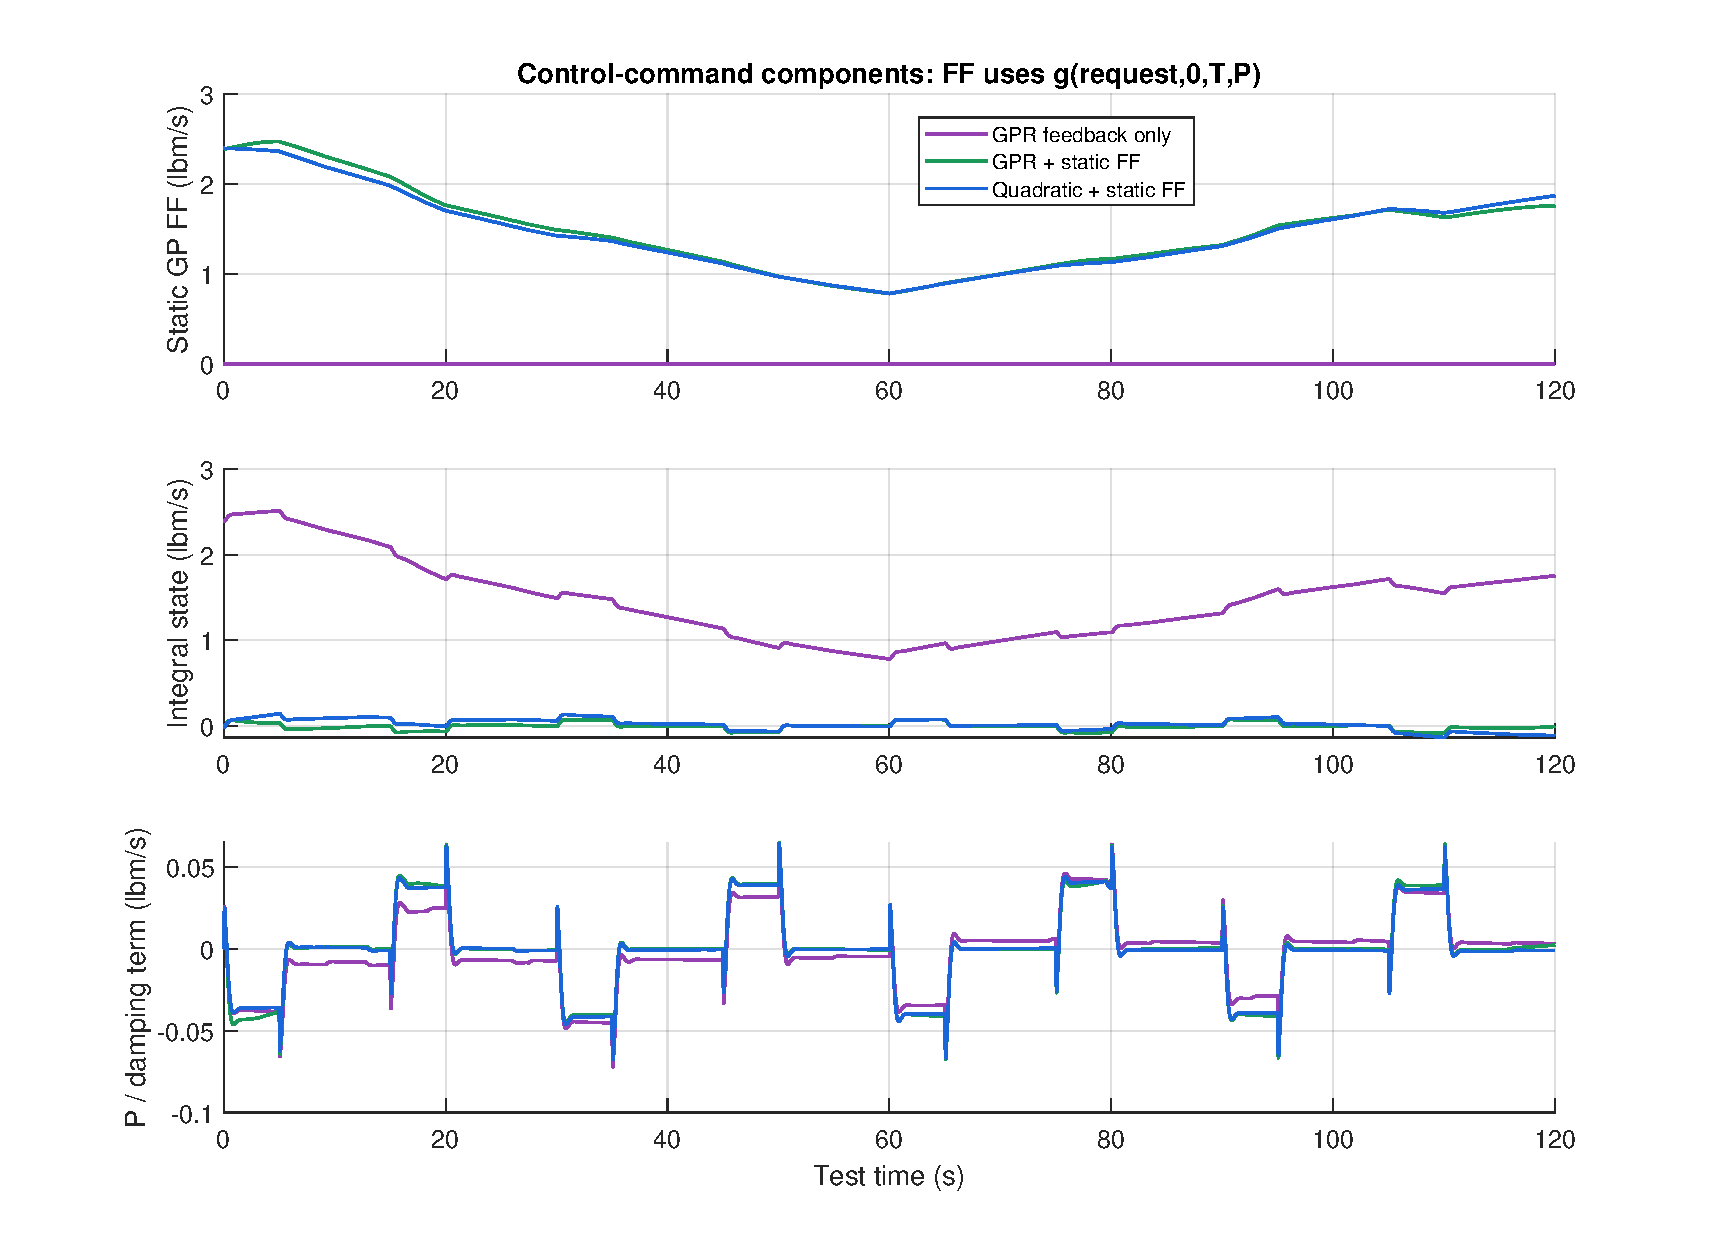
\includegraphics[width=\linewidth]{static_ff_components.pdf}\caption{GPR and quadratic command components, with the GPR feedback-only case retained for context.}\end{figure}
Static model bias can be absorbed by the residual integral at a settled operating point. During changing ambient conditions and speed ramps, the model's value and slope errors can alter that compensation. The plots show the measured command decomposition; they should be interpreted together with actual-speed RMSE and fuel reversal rather than treating a smaller integral state as a performance result.
\section{Reproduction}
The challenger is \path{GasTurbine_PolyCompare_R3_Poly2FF.mdl}, with setup \path{tmats_r3_poly2_setup.m}. The three comparator models use the same \path{GasTurbine_PolyCompare_} prefix. Run \path{fit_tmats_poly2_inverse.py}, \path{validate_tmats_poly2.m}, and \path{run_tmats_r3_cycle(out,true,true,true)} with \path{out='results/r3_poly2_challenger_20260915'}. The fitted equation and normalization are stored in \path{results/poly2_inverse_20260915/poly2_model.json}.

Run \path{audit_tmats_cycle_coverage(out)}, \path{report_tmats_static_ff(out)} and \path{verify_tmats_static_ff.py poly} for the coverage audit, figures and independent checks. The archive contains the fitted equation, held-out predictions, new models, native trajectories and summary tables. It requires the existing T-MATS workspace and frozen-model dependencies.
\end{document}
